\documentclass{beamer}

%\usepackage{subfigure}
\usepackage{graphicx}
\usepackage{sidecap}
\usepackage{caption}
\usepackage{subcaption}
\captionsetup{compatibility=false}
\usepackage{appendixnumberbeamer}
\usepackage{amsmath}
% --
\usepackage{multirow}
\usepackage{xcolor}
\usepackage{setspace}
\usepackage{hyperref}
\usepackage{anyfontsize}

\beamertemplatenavigationsymbolsempty
\setbeamertemplate{footline}

\newenvironment{itemise} {\begin{itemize} \setlength{\itemsep}{0.2cm}} {\end{itemize}}
\usepackage[labelformat=empty]{caption}
\setbeamertemplate{sections/subsections in toc}[square]

%% COLORS
\definecolor{Gray}{gray}{0.9}
\definecolor{dblue}{rgb}{0.132,0.1,0.27}
\definecolor{mint}{cmyk}{1.0, 0.2, 0.6, 0.05}
\definecolor{ant}{cmyk}{0.5, 0.1, 0.0, 0.45}
\definecolor{lgray}{cmyk}{0.12, 0.0, 0.0, 0.17}
\definecolor{lred}{cmyk}{0.0, 0.9, 0.7, 0.0}


\usepackage{etoolbox}% http://ctan.org/pkg/etoolbox 
\usepackage{booktabs}

\newenvironment{literatur}{%
  \parskip2pt \parindent0pt \raggedright
  \def\lititem{\hangindent=0.5cm \hangafter1}}{%
  \par\ignorespaces}

\newcommand{\tb}[1]{{\color{blue}{\textbf{#1}}}}
\newcommand{\tm}[1]{{\color{mint}{\textbf{#1}}}}
\newcommand{\tr}[1]{{\color{red}{\textbf{#1}}}}
% Ilya: packages

\usepackage{tikz}
\usepackage{lmodern}
\usepackage{enumitem}

% Ilya: my commands

\newenvironment{mytemize}
{\vfill\itemize[nolistsep,itemsep=\fill,label=\color{blue}{$\triangleright$}]}
  {\enditemize}


\newenvironment{mynumerate}
{\vfill\enumerate[nolistsep,itemsep=\fill,label=\arabic*.]}
  {\endenumerate}

\newcommand{\hitem}[1]{
  {\color{blue}{$\triangleright$}} 
  {#1} 
  {\hfill}
}

\setlist[itemize]{label= \color{blue}{$\triangleright$}}
\setlist[enumerate]{label = \arabic*.}

\newcommand{\rarr}{$\Rightarrow$\ }

%------------------------------------------------------------------------------------
% TITLE
%------------------------------------------------------------------------------------
\title[PSME]{Macroeconomics\\ Lecture 9 -- Small Open Economy RBC; Large Open Economy}
\author[I. Eryzhenskiy]{Ilya Eryzhenskiy}
\institute[Paris-1]{PSME Panth\'{e}on-Sorbonne Master in Economics}
\date[PSME macro]{Fall 2023}

%---BEGIN------------------------------------------------------------------------------
\begin{document}
%---BEGIN------------------------------------------------------------------------------
\begin{frame}
\maketitle
\end{frame}
%---FRAME------------------------------------------------------------------------------
%\section{Outline}
\begin{frame}
\frametitle{Outline}
\tableofcontents
\end{frame}

\begin{frame}{Capital, Balance of payments and IIP}
  In a small open economy with capital:  
  \begin{mynumerate}
  \item investment affects trade balance: $TB_t = Y_t - C_t - I_t$
	\begin{mytemize}
	  \item[\rarr] Effect of temporary productivity shock on TB and CA now ambiguous: both $C_t$ and $I_t$ rise and counteract larger $Y_t$
	\end{mytemize}
  \item household savings channelled to both investment and foreign assets: $\Omega_{t+1} - \Omega_t = I_t + IIP_{t+1} - IIP_t$
	\begin{mytemize}
	  \item[\rarr] consumption-saving choice does not fully explain the CA
	\end{mytemize}
  \end{mynumerate}
\end{frame}


\section{Real Business Cycles in Small Open Economy (SOE RBC)}

\begin{frame}
\frametitle{Outline}
\tableofcontents[currentsection]
\end{frame}

\begin{frame}{A SOE RBC model}
  The RBC framework extended to include exchanges with the rest of the world:
  \begin{mynumerate}
  \item Foreign assets held instead of domestic bonds \rarr \tb{IIP} variable
  \item Exogenous interest rate \rarr steady state existence and stability problem \rarr an additional assumption on foreign asset holding is needed 
	\begin{mytemize}
	  \item we focus on \tb{interest rate premium}, or external debt-elastic interest rate (EDEIR) assumption
	\end{mytemize}
    \item \tb{Capital adjustment cost} limits volatility of investment \rarr limits volatility of \tb{trade balance}
  \end{mynumerate}
\end{frame}

\begin{frame}{Household Problem (in Social Planner form)}
\begin{equation*}
\label{eq:soe-rbc-utility-edeir}
\max_{C_t, N_t, IIP_{t+1}, K_{t+1}} E_0 \sum_{t=0}^{\infty} \beta^t u(C_t,N_t)
\end{equation*}
subject to
\begin{equation*}
\label{eq:soe-rbc-bc-edeir}
C_t + K_{t+1} - (1-\delta) K_t + IIP_{t+1} + \Phi(K_{t+1}-K_t) = 
A_t F(K_t,N_t)+ (1+r_{t-1})IIP_{t}
\end{equation*}
\begin{equation*}
  K_0, IIP_0 \ \ \text{-- given}; \quad \ln A_{t} = \rho \ln A_{t-1} +  \epsilon_{t}
  \label{eq:init}
\end{equation*}

\vfill
$\Phi(\cdot)$ is a convex \tb{capital adjustment cost} function with $\Phi(0)=\Phi'(0) =0$; $\Phi''(\cdot)>0 $
\vfill
Notice a (yet) another type of utility function: non-separable, with labor and not leisure as argument: $u(\underset{+}{C_t}, \underset{-}{N_t})$ 
%A transversality condition for IIP applies:  $\lim_{j \rightarrow \infty} E_t \frac{IIP_{t+j}}{\prod_{s=0}^j(1+r_s)} \geq 0 $

\end{frame}

\begin{frame}{Planner's FOC}
  $\frac{\partial \mathcal L}{\partial C_t}$:
\begin{equation*}
\label{eq:soe-rbc-foc-c-edeir}
 u'_C(C_t,N_t)
= \lambda_t 
\end{equation*}
$\frac{\partial \mathcal L}{\partial IIP_{t+1}}$:
\begin{equation*}
\label{eq:soe-rbc-foc-d-edeir}
\lambda_t = \beta (1+r_{t})E_t\lambda_{t+1}
\end{equation*}
$\frac{\partial \mathcal L}{\partial N_{t}}$:
\begin{equation*}
\label{eq:soe-rbc-foc-h-edeir}
-u'_N(C_t,N_t) = \lambda_t A_t F'_N(K_t,N_t)
\end{equation*}
$\frac{\partial \mathcal L}{\partial K_{t+1}}$:
\begin{align*}
\label{eq:soe-rbc-foc-k-edeir}
1+\Phi'(K_{t+1}-K_t)
= \beta
E_t \frac{\lambda_{t+1}}{\lambda_t }
&\left[
A_{t+1} F'_K(K_{t+1}, N_{t+1})
+ \right.\\ &\left.1-\delta + \Phi'(K_{t+2}-K_{t+1})
\right]
\end{align*}
$\frac{\partial \mathcal L}{\partial \lambda_t}$:
\begin{equation*}
\label{eq:soe-rbc-bc-combined-edeir}
C_t + K_{t+1}-(1-\delta)K_t+ IIP_{t+1}+\Phi(K_{t+1}-K_t) 
= A_t F(K_t,L_t)+ (1+r_{t-1})IIP_t
\end{equation*}
 
\end{frame}

\begin{frame}{Interest Rate Premium/ EDEIR}
  \tb{External debt-Elastic Interest Rate (EDEIR)}: for this model it is mostly a trick to achieve existence and stability of steady state. \\
\begin{equation*}
\label{eq:soe-rbc-r-edeir}
r_t = r^* + p(\underset{-}{IIP_t})
\end{equation*}
\begin{mytemize}
\item $r^*=$ world interest rate, assumed  \textbf{constant}\\
\item $p(IIP_t)=$  country interest-rate premium, decreasing in IIP (increasing in external debt)
  \begin{mytemize}
  \item intuition: high debt \rarr repayment risk \rarr premium
  \end{mytemize}
\item "External" means that \textbf{the household takes the premium as given} i.e. we do not use the function when obtaining $\frac{\mathcal{L}}{IIP_{t+1}}$
\end{mytemize}
%\\
%$\tilde{d}_t=$ cross-sectional average of debt

%In equilibrium cross-sectional average of debt must equal individual debt 
%\begin{equation*}
%\label{eq:edeir-dtilde=d}
%\widetilde{d}_t = d_t
%\end{equation*}
\end{frame}

\begin{frame}{Balance of Payments Indicators}
\tb{Trade Balance}
\begin{equation*}
\label{eq:soe-rbc-tb-edeir}
TB_t =Y_t-C_t - I_t - \Phi(K_{t+1}-K_t)
\end{equation*}

\tb{Current Account}
\begin{equation*}
\label{eq:soe-rbc-ca=tb-rd-edeir}
CA_t = TB_t + r_{t} IIP_t
\end{equation*}
\end{frame}

\begin{frame}{Equilibrium}

An equilibrium is a sequence $\{C_t, L_t, K_{t+1}, IIP_{t+1}\}$, such that, given exogenous initial conditions $K_0, IIP_0, A_0$ and exogenous productivity $\ln A_{t+1} = \rho \ln A_t + \widetilde{\eta}  \epsilon_{t+1}
$, the following conditions are satisfied:
\begin{equation*}
\label{eq:soe-rbc-foc-d-eqm-edeir}
u'_C(C_t,L_t) = \beta (1+r^* + p(IIP_{t+1}))E_t  u'_C(C_{t+1},L_{t+1})
\end{equation*}
\begin{equation*}
\label{eq:soe-rbc-uh/uc-edeir}
-\frac{u'_L(C_t,L_t)}{u'_C(C_t,L_t)}
= A_t f'_L(K_t,L_t)
\end{equation*}
\vfill
\begin{equation*}
\hspace{-0.5cm}
\label{eq:soe-rbc-foc-k-eqm-edeir}
1= \beta
E_t \left\{%\left\{ 
  \frac{ u'_C(C_{t+1},L_{t+1})}{ u'_C(C_t,L_t)}
\frac{
A_{t+1}f'_K(K_{t+1},L_{t+1})
+1-\delta + \Phi'(K_{t+2}-K_{t+1})
}{1+\Phi'(K_{t+1}-K_t)
}\right\}
%\right\}
\end{equation*}
\vfill
\begin{align*}
C_t+ K_{t+1}-(1-\delta) K_t + IIP_{t+1}&+\Phi(K_{t+1}-K_t)\\
& =A_t f(K_t,L_t)+ IIP_{t} (1+r^*+p(IIP_t)) 
\end{align*}
 
\end{frame}

\begin{frame}{Steady State}

The steady state $(IIP, K, C , L)$ is solution to a system (with $A=1$): 

\begin{equation*}
\label{eq:soe-rbc-uh/uc-edeir_ss}
-\frac{u'_L(C,L)}{u'_C(C,L)}
= A f'_L(K,L)
\end{equation*}
\begin{equation*}
\label{eq:soe-rbc-bc-combined-eqm-edeir_ss}
C+ \delta K - IIP\cdot(r^*+p(IIP))  
=A f(K,L) 
\end{equation*}
\begin{equation*}
\label{eq:soe-rbc-foc-d-eqm-edeir_ss}
1 = \beta (1+r^* + p(IIP))
\end{equation*}
\begin{equation*}
\label{eq:soe-rbc-foc-k-eqm-edeir_ss}
1= \beta
\left[
A f'_K(K,L)
+1-\delta  
\right]
\end{equation*}

\end{frame}

\begin{frame}{Balance of Payments in Steady State}
  Recall $IIP_{t+1} - IIP_t = CA_t$ from previous lecture. \\ Since $IIP_t = IIP$ (constant)  in s.s., $CA = 0$ in s.s.
  \vfill
  Recall then $CA = TB + r \cdot IIP$ \rarr $TB = - r \cdot IIP$.
  \vfill
  \underline{Intuition:} net \tb{capital flows (FA balance)} are null in s.s., so the flows due to \tb{trade balance} are exactly compensated by flows due to \tb{income balance}, for \tb{Balance of Payments Identity} $CA = FA$ to hold.
  
\end{frame}

\begin{frame}{Functional Forms}

{Instantaneous utility function -- GHH } 
\[
u(C,L) = 
\frac{
\left(
C-L^{\omega}/\omega
\right)^{1-\sigma}
-1
}
{1-\sigma};
\quad \omega>1; \sigma>0
\]
\tr{\rarr labor supply depends on real wage only (not on consumption)} \\

{Interest rate premium} 
\[
p(IIP) = \psi \left(e^{\bar{IIP}- IIP} -1 \right); \quad \psi >0 
\]
{Production function -- Cobb-Douglas}
\[
f(K,L) = K^{\alpha}L^{1-\alpha}; \quad \alpha \in (0,1)
\]
{Adjustment cost function -- quadratic}
\[
\Phi(x) = \frac{\phi}{2} x^2; \quad \phi>0
\]
6 structural parameters: $\sigma$, $\omega$, $\psi$, $\bar{IIP}$, $\alpha$, $\phi$
\end{frame}

\begin{frame}{Euler equation in small open economy}
    $$u'_C(C_t, N_t) = \beta $$
\end{frame}

\begin{frame}{Steady State}
  using the assumed functional forms,  
  the steady state $(IPP, K, C , L)$ is solution to a system (with $A=1$): 
\begin{equation*}
\label{eq:soe-rbc-uh/uc-edeir_ss'}
L^{\omega -1}
= A (1-\alpha) (K/L)^{\alpha}
\end{equation*}
\begin{equation*}
\label{eq:soe-rbc-bc-combined-eqm-edeir_ss'}
C+ \delta K - (r^*+ \psi(e^{\bar{IIP}- IIP}))  IIP
=A (K/L)^{\alpha } L 
\end{equation*}
\begin{equation*}
1 = \beta (1+r^* + \psi(e^{\bar{IIP}- IIP }-1))
\end{equation*}
\begin{equation*}
1= \beta
\left[
A \alpha (K/L)^{\alpha -1}
+1-\delta  
\right]
\end{equation*}
\textbf{7} parameters in the s.s. system: $\omega, \alpha, \delta, r^*, \psi,  \bar{d}, \beta$. 
\textbf{+ 4} more parameters in model, eliminated in s.s.: $\sigma$, $\phi$, $\rho$, $\tilde{\eta}$
\end{frame}

\section{Calibration/estimation}
\begin{frame}
\frametitle{Outline}
\tableofcontents[currentsection]
\end{frame}
\begin{frame}{Calibration/estimation strategy}

Three categories of parameters have different calibration approaches: \\
\vfill
\underline{Category a:} manual calibration based on literature consensus/more arbitrary arguments;  {\bf 4} parameters: $\sigma=2$, $\delta=0.1$, $r^*=0.04$, $\beta=1/(1+r^*)$. 
\\
\vfill
\underline{Category b:} restrictions to match \tb{first moments}  (\tr{averages}) of the data that the model aims to explain, {\bf 2} parameters:  $\alpha$, $\overline{d}$
\begin{align*}
\mbox{labor share } =& 0.68\\
\mbox {trade-balance-to-output ratio } = & 0.02
\end{align*}
\vfill
\underline{Category c:} restrictions to match \tb{second moments}  (\tr{variances, correlations}) of the data that the model aims to explain, {\bf 5} parameters:  $\omega$, $\phi$,  $\psi$, $\rho$,  $\tilde{\eta}$. The second moments to be matched are: 
$\sigma_y$, $\sigma_L$, $\sigma_I $, $\sigma_{TB/Y}$, corr$(\ln Y_t, \ln Y_{t-1})$ 
\end{frame}


\section{Model Outputs}
\begin{frame}
\frametitle{Outline}
\tableofcontents[currentsection]
\end{frame}
\begin{frame}{Calibration/estimation -- parameter values}
  Assume that one \textbf{period} is \textbf{one year}; calibrate the model to the \tr{Canadian economy}. 
  \vfill

\begin{tabular}{|c|c|c|c|c|c|c|c|c|c|}
\hline
$ \sigma$&
$r^*$&
$\delta$&
$\alpha$&
$ \omega$&
$\phi$&  
$\rho$& 
$\sigma_{\epsilon}$&$\bar{IIP}$&
$\psi$\\
\hline
  2 & 
0.04&
0.1&
0.32&
1.455 &
0.028&
0.42&
0.013
&
-0.744& 0.0007  
\\
\hline
\end{tabular}

\vfill
$\beta$ follows from $r^*$: $1/\beta = 1+r^*$ from Euler equation.
\vfill
Given parameter values,  the steady state can be computed with any software that solves non-linear systems: %using the  Matlab program \verb7edeir_ss.m7 available on the book's Website. This yields

\centerline{\begin{tabular}{|c|c|c|c|}
 \hline 
$C$&$IIP$&$L$&$k$\\
\hline 
    1.1170
&   -0.7442
&   1.0074
&    3.3977\\
\hline 
\end{tabular}
}
\end{frame}

%\begin{frame}{Canadian Economy: Second-order Moments}
%\centerline{\small
%\begin{tabular}{|c|c|c|c|}
%\hline
%Variable&\multicolumn{3}{|c|}{Canadian Data}\\
%\cline{2-4}
%&$\sigma_{x_t}$
%&$\rho_{x_t,x_{t-1}}$
%&$\rho_{x_t,GDP_t}$
%\\
%\hline
%$y$           &  2.8&  0.61&      1\\
%$C$           &  2.5&   0.7&   0.59\\
%$I$           &  9.8&  0.31&   0.64\\
%$L$           &    2&  0.54&    0.8\\
%$\frac{TB}{y}$&  1.9&  0.66&  -0.13\\
%\hline
%\end{tabular}}
%
%\centerline{\tiny Source: Mendoza AER, 1991. Annual data. Log-quadratically detrended.}
%
%
%\begin{itemize}
%\item Volatility ranking:
%$\sigma_{TB/y}<$$\sigma_C<$$\sigma_y<$$\sigma_I$. 
%\item Consumption, investment, and hours are \tb{procyclical}. 
%\item The trade-balance-to-output ratios is \tb{countercyclical}. 
%\item All variables considered have a positive autoregressive coefficient. 
%\item Similar patterns for other \textit{developed} SOEs. 
%\end{itemize}
%
%
%\end{frame}

\begin{frame}{Positive Productivity Shock -- impulse responses} 

%\label{fig:mendoza91} 


\centering
\includegraphics[width = 0.85\linewidth]{FIGURES/RBC_} 


\end{frame}

\section{Comparative Statics of Model}

\begin{frame}
\frametitle{Outline}
\tableofcontents[currentsection]
\end{frame}


\begin{frame}{Response of TB and varying capital adjustment cost}

\begin{center}
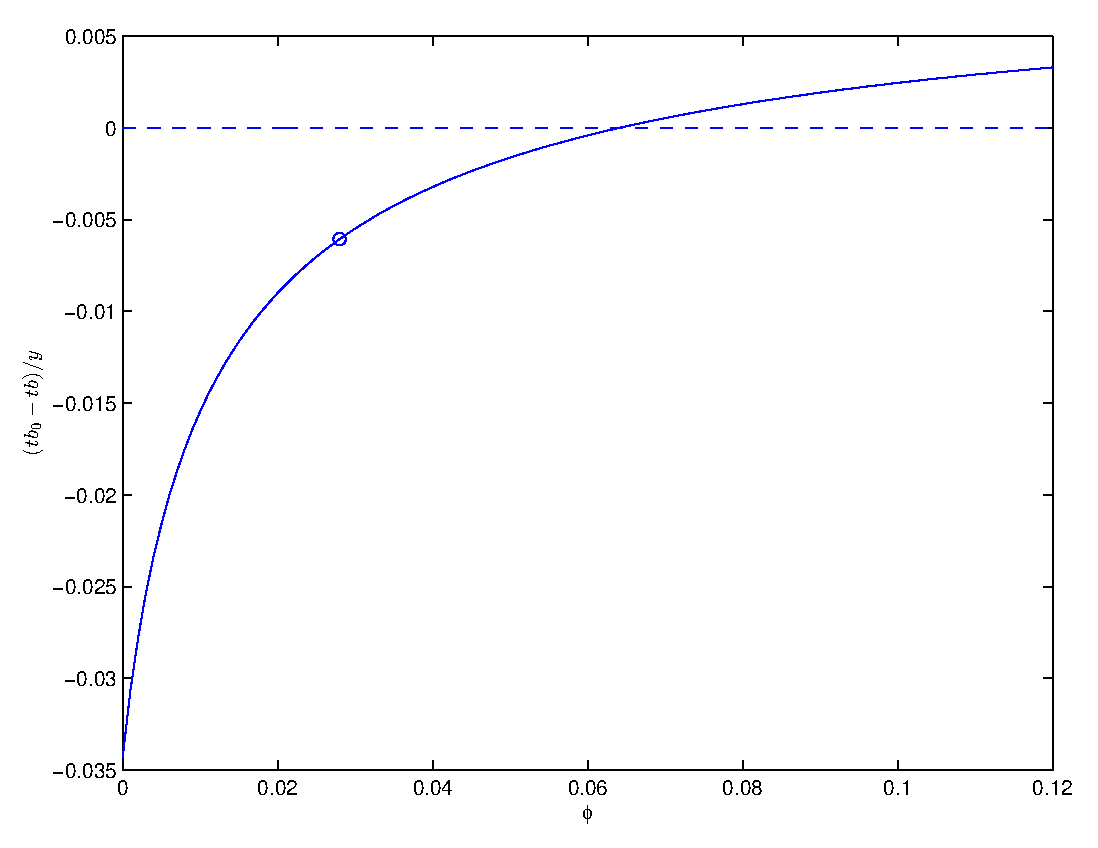
\includegraphics[width = 0.7\linewidth]{FIGURES/soe_rbc_irtbys_phi_slides.eps} 
\end{center}
\vspace{-0.5cm}
%Produced with: Z:\uribe\book\soe_rbc\edeir\edeir_sensitivity\edeir_run.m
Higher capital adj. costs \rarr more positive impulse response of TB. For $\phi<0.06$ (scale parameter of adj. cost), the response of the trade balance negative.
\\
Recall $TB_t = Y_t - C_t - I_t$. With large adj. cost, investment response weak \rarr consumption drives TB \rarr intuition from 2-period model with consumption only applies.

\end{frame}


\begin{frame}{Response of TB and varying productivity persistence}

\begin{center}
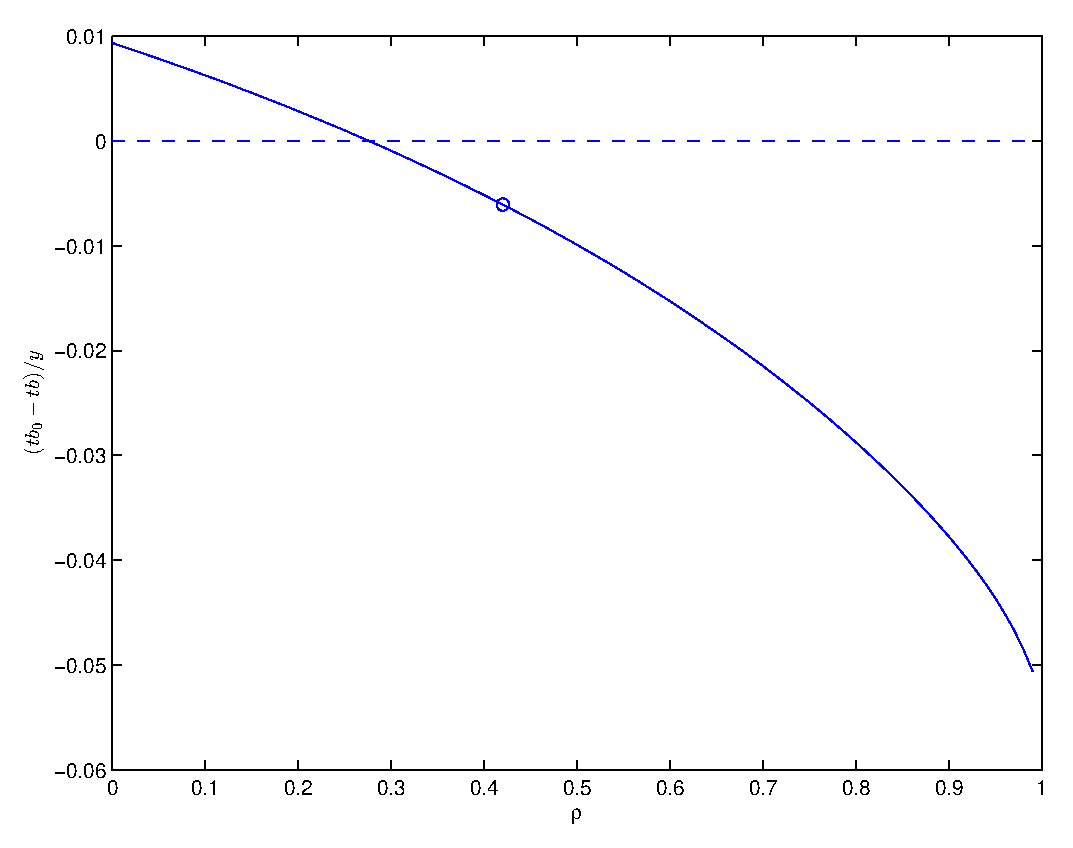
\includegraphics[width = 0.7\linewidth]{FIGURES/soe_rbc_irtbys_rho_slides.eps} 
\end{center}
\vspace{-0.5cm}
%Produced with: Z:\uribe\book\soe_rbc\edeir\edeir_sensitivity\edeir_run.m
More persistent the productivity shock \rarr smaller impulse response of TB (recall temporary vs. permanent shocks in the 2-period model). For $\rho>0.3$ (productivity persistent enough), the response of TB is negative.

\end{frame}



\section{Business Cycles in a Small Open Economy: Data}

\begin{frame}{Canadian Economy: Business-Cycle Statistics}
  Canada -- developed economy, but 2.1 \% of world GDP \rarr ``small'' (compare to China -- 18.4\%; USA -- 24\% -- large open economies). 
  \vfill
  We will seek to explain historical business-cycle patterns: 1946-1985.
  \vfill
\centerline{
\begin{tabular}{|c|c|c|c|}
\hline
Variable ($x_t$)&\multicolumn{3}{|c|}{Moments}\\
\cline{2-4}
&$\sigma_{x_t}$
&corr$(x_t,x_{t-1})$
&corr$(x_t,Y_t)$
\\
\hline
$Y$           &  2.8&  0.61&      1\\
$C$           &  2.5&   0.7&   0.59\\
$I$           &  9.8&  0.31&   0.64\\
$L$           &    2&  0.54&    0.8\\
$\frac{TB}{Y}$&  1.9&  0.66&  -0.13\\
\hline
\end{tabular}}

\centerline{\tiny Source: Mendoza AER, 1991. Annual data. Log-quadratically detrended.}


\end{frame}

\begin{frame}{Canadian Economy: Business-Cycle Patterns}
\begin{mytemize}
\item Volatility ranking:
$\sigma_{TB/Y}<$$\sigma_C<$$\sigma_Y<$$\sigma_I$. 
\item Consumption, investment, and labor hours are \tb{procyclical}. 
\item The trade-balance-to-output ratio is \tb{countercyclical}. 
\item All variables have a positive autoregressive coefficient. 
\item Similar patterns hold for other \textit{developed} SOEs. 
\end{mytemize}

\end{frame}


\begin{frame}{Second-order Moments: RBC vs. Data}


{\small
\begin{center}
\begin{tabular}{|c|ccc|ccc|ccc|}
\hline
&\multicolumn{3}{c|}{Canada, 1960-2011}&\multicolumn{3}{|c|}{Model}\\
&$\sigma_{x_t}$ &$corr(x_t,x_{t-1})$ &$corr(x_t,Y_t)$ 
&$\sigma_{x_t}$ &$corr(x_t,x_{t-1})$ &$corr(x_t,Y_t)$
\\
 \hline
$Y$  
&   3.7&  0.9&  1
&  3.1 &  0.6&  1
\\
$C$ & 2.2&  0.7&  0.6
&  2.7&  0.8&  0.8
\\
$I$ &  10.3&  0.7&  0.8
&  9.0&  0.1&  0.7
\\
$N$     &   3.6&  0.7&  \tm{0.8}
&  2.1&  0.6&  \tr{1}
\\
$\frac{TB}{Y}$  &   1.7&  0.8&  0.1
&  1.8&  0.5&  -0.04
\\
\hline
\end{tabular}
\end{center}

}


\begin{mytemize}
\item   $\sigma_L$, $\sigma_I$, $\sigma_Y$,
$\sigma_{TB/Y}$, and $\rho_{Y_t,Y_{t-1}}$  were targeted by calibration, so no real test  here.  

\item As before, the model correctly ranks $\sigma_C < \sigma_Y < \sigma_I$. The trade balance (normalized by GDP) correctly has $\sigma_{TB/Y}$ < $\sigma_Y$

\item  model correctly makes $TB/Y$ \tb{countercyclical}. 

\item   model \tr{overestimates} the correlations of hours and consumption with output (due to GHH utility). 
 
\end{mytemize}


\end{frame}

\section{Current account in partial equilibrium} 

\begin{frame}{$C$, $I$ and interest rate: partial equilibrium}
  We now consider the \textbf{partial equilibrium} effect of $r_{t+1}$ on $CA_t$, through $C_t = C(r_{t}, \dots)$ and $I_t = I(r_{t}, \dots)$.
  \vfill
  Recall that interest rate influences consumption through substitution effect and income effect.
  \begin{mynumerate}
  \item Substitution effect: higher $r_{t+1}$ \rarr $C_{t+1}$ relatively cheaper with respect to $C_t$ \rarr $C_t$ decreases (seen in Dynamic IS eq.)
  \item Income effect: less savings needed to guarantee a given level of $C_{t+1}$ \rarr $C_t$ might increase
  \end{mynumerate}

  \textbf{Assume substitution effect dominates} (e.g. if $u(C) = \ln(C)$), then $C_t = C_t(\underset{-}{r_{t}}, \dots)$
  \vfill 
  Furthermore, $I_t = I(\underset{-}{r_{t}}, \dots)$, because firms' optimal $K_{t+1}$ depends negatively on $R_{t+1}$ and $r_t$ is positively correlated with $R_{t+1}$ in equilibrium.
\end{frame}

\begin{frame}{Trade balance, Current account in parial equilibrium}

We get a \textbf{positive dependence of both TB and CA on real interest rate}:
      $$TB_t = Y_t - C(\underset{-}{r_{t}},\dots) - I(\underset{-}{r_{t}}, \dots)= TB(\underset{+}{r_{t}},\dots)$$
      $$CA_t = \underbrace{Y_t - C(\underset{-}{r_{t}},\dots) - I(\underset{-}{r_{t}}, \dots)}_{TB_t} +  r_{t-1} IIP_t = CA(\underset{+}{r_{t}},\dots)$$
\end{frame}

\begin{frame}{Current account schedule}
  \begin{columns}
	\column{0.5\textwidth} CA schedule -- positively sloped line/curve in $(CA, r)$ space (time indexes dropped).\\
	\vfill
  Shifted by all the factors other than $r$ that affect current account, e.g.:
  \begin{mytemize}
	\item Productivity 
	\item Household wealth 
	\item Preferences
  \end{mytemize}
\column{0.5\textwidth} 
  \end{columns}
  \end{frame}

\begin{frame}
\frametitle{Outline}
\tableofcontents[currentsection]
\end{frame}

\begin{frame}{Risk premium}
  \begin{columns}
	\column{0.5\textwidth} 
	Heavily indebted economies might be bad borrowers \rarr market imposes a \tb{risk premium}. Simple modelling approach: 

	$$r = r^* + \underbrace{p(\underset{-}{CA})}_{\text{premium}}$$
  
  Plot function together with CA schedule $\rightarrow$ graphical solution of equilibrium $r, CA$
\column{0.5\textwidth} 
  \end{columns}
\end{frame}

\section{Large Open Economy -- Patial Equilirium}

\begin{frame}{Large open economy}
  Assume only two economies/economic zones in the world. Typical application: one big open economy $+$ rest of the world as another ``economy''.
\vfill
  \tb{Large open economy} can influence world prices. We have focused on one price in this lecture: real interest rate.  
  \vfill 
  World interest rate will be determined by two large open economies' CA schedules.
  \vfill
  Equilibrium condition $CA^A(r) = -CA^B(r)$: all outflows from one country are inflows in the other (nothing else in the world!)
\end{frame}

\begin{frame}{Large open economy partial equilibrium: graph}
  
\end{frame}

\section{Global savings glut}
\begin{frame}
\frametitle{Outline}
\tableofcontents[currentsection]
\end{frame}

\begin{frame}{Persistent CA deficits in US}
  U.S. current account has been in persistent deficit since 1970s:
  \begin{figure}
	\centering
	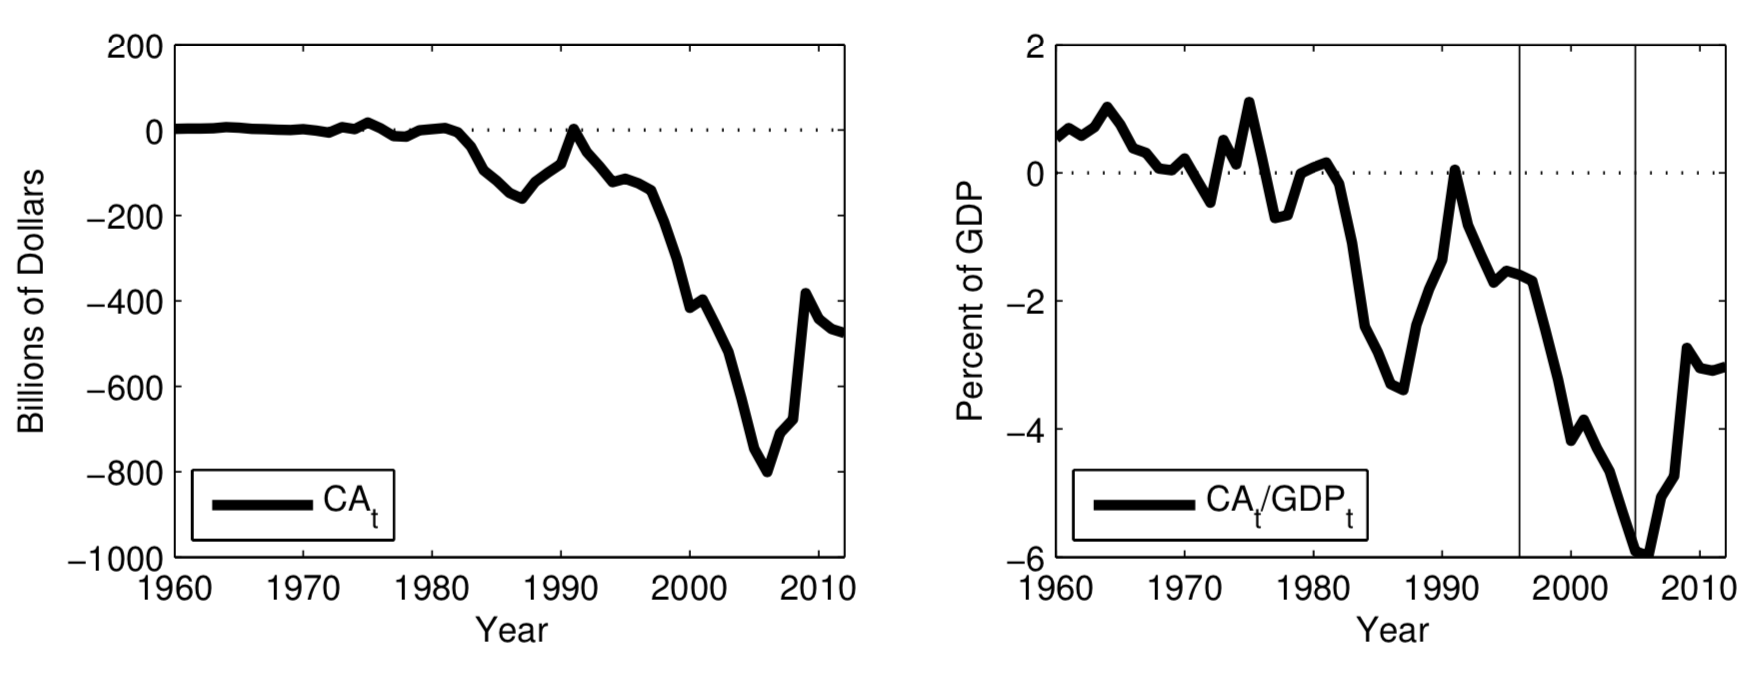
\includegraphics[width = 0.99\textwidth]{FIGURES/CA_US.png}
  \end{figure}
  \vspace{-0.5cm}
  \begin{minipage}{\columnwidth}
  \footnotesize
  Source: Schmitt-Grohe, Uribe, Woodford, Fig. 6.9
  \end{minipage}
\end{frame}

\begin{frame}{Hypotheses for the CA deficits}
  \begin{mynumerate}
  \item ``Made in the U.S.A.'' -- common view in early 2000s
	\begin{mytemize}
	\item Abnormal consumption, e.g. due to developed consumer credit markets
	\item Investment bubbles
	\end{mytemize}
  \item ``Global Savings Glut'' -- B. Bernanke (2005)
	\begin{mytemize}
	\item Developing economies accumulate foregn reserves in the aftermath of crises of 1970s and 1990s
	\item Export-led growth through currency depreciations
	\end{mytemize}
  \end{mynumerate}
  \vfill
  \textbf{Which one is right?} Look at the large open economy model and at data.
\end{frame}

\begin{frame}{Made in U.S.A. vs. Global Savings Glut -- diagrams} 
  
\end{frame}

\begin{frame}{World real interest rate}
  \begin{figure}
	\centering
	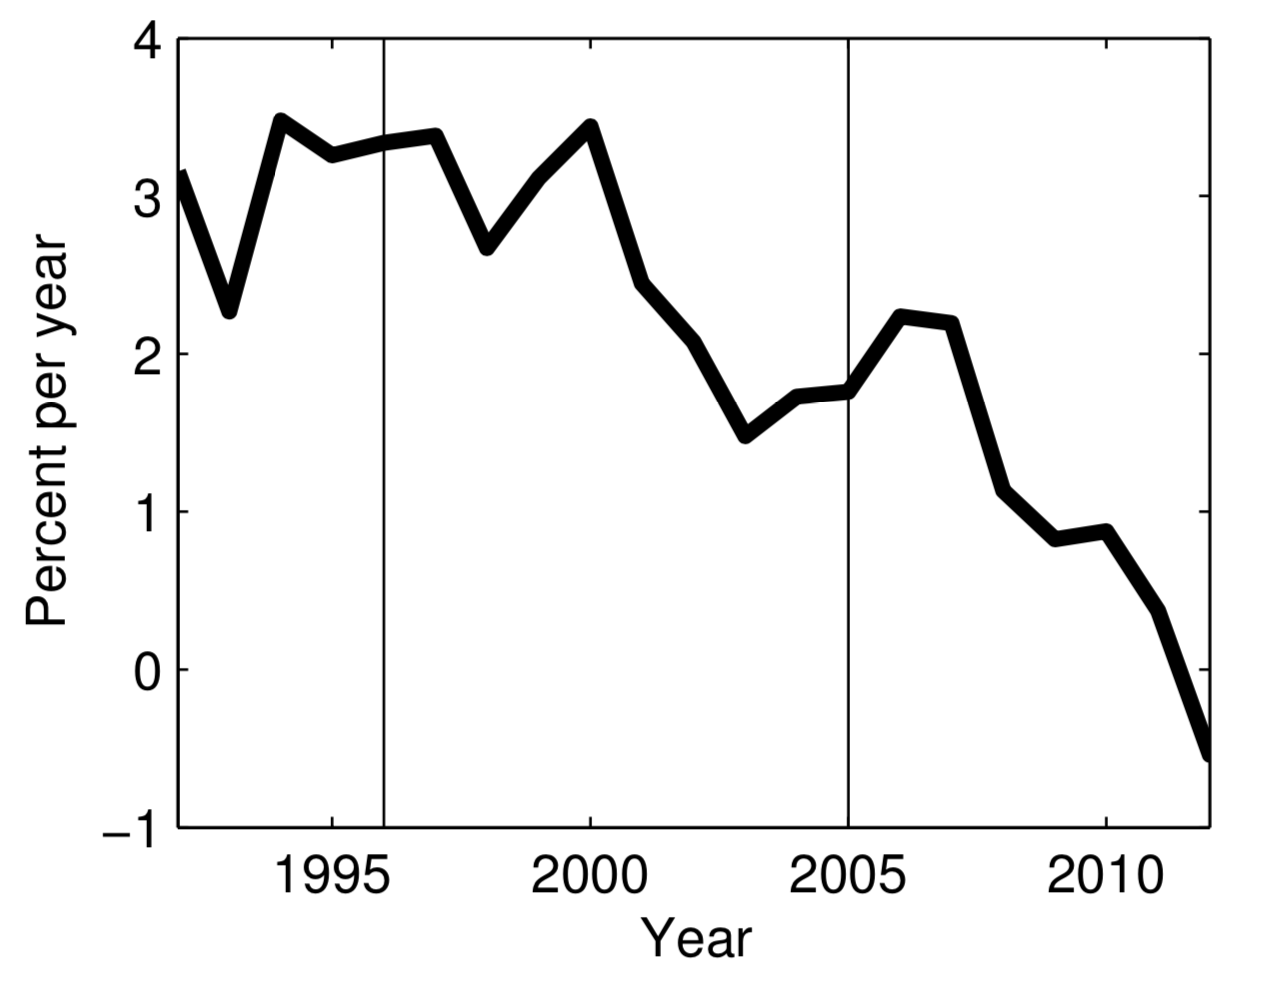
\includegraphics[width = 0.8\textwidth]{FIGURES/world_int_rate.png}
  \end{figure}
  \vspace{-0.5cm}
  \begin{minipage}{\columnwidth}
  \footnotesize
  Source: Schmitt-Grohe, Uribe, Woodford, Fig. 6.11
  \end{minipage}
  \centering
  \alert{Congratulations, prof. Bernanke!}
\end{frame}

\end{document}
